% Options for packages loaded elsewhere
\PassOptionsToPackage{unicode}{hyperref}
\PassOptionsToPackage{hyphens}{url}
\PassOptionsToPackage{dvipsnames,svgnames,x11names}{xcolor}
%
\documentclass[
  letterpaper,
  DIV=11,
  numbers=noendperiod]{scrartcl}

\usepackage{amsmath,amssymb}
\usepackage{iftex}
\ifPDFTeX
  \usepackage[T1]{fontenc}
  \usepackage[utf8]{inputenc}
  \usepackage{textcomp} % provide euro and other symbols
\else % if luatex or xetex
  \usepackage{unicode-math}
  \defaultfontfeatures{Scale=MatchLowercase}
  \defaultfontfeatures[\rmfamily]{Ligatures=TeX,Scale=1}
\fi
\usepackage{lmodern}
\ifPDFTeX\else  
    % xetex/luatex font selection
\fi
% Use upquote if available, for straight quotes in verbatim environments
\IfFileExists{upquote.sty}{\usepackage{upquote}}{}
\IfFileExists{microtype.sty}{% use microtype if available
  \usepackage[]{microtype}
  \UseMicrotypeSet[protrusion]{basicmath} % disable protrusion for tt fonts
}{}
\makeatletter
\@ifundefined{KOMAClassName}{% if non-KOMA class
  \IfFileExists{parskip.sty}{%
    \usepackage{parskip}
  }{% else
    \setlength{\parindent}{0pt}
    \setlength{\parskip}{6pt plus 2pt minus 1pt}}
}{% if KOMA class
  \KOMAoptions{parskip=half}}
\makeatother
\usepackage{xcolor}
\setlength{\emergencystretch}{3em} % prevent overfull lines
\setcounter{secnumdepth}{5}
% Make \paragraph and \subparagraph free-standing
\makeatletter
\ifx\paragraph\undefined\else
  \let\oldparagraph\paragraph
  \renewcommand{\paragraph}{
    \@ifstar
      \xxxParagraphStar
      \xxxParagraphNoStar
  }
  \newcommand{\xxxParagraphStar}[1]{\oldparagraph*{#1}\mbox{}}
  \newcommand{\xxxParagraphNoStar}[1]{\oldparagraph{#1}\mbox{}}
\fi
\ifx\subparagraph\undefined\else
  \let\oldsubparagraph\subparagraph
  \renewcommand{\subparagraph}{
    \@ifstar
      \xxxSubParagraphStar
      \xxxSubParagraphNoStar
  }
  \newcommand{\xxxSubParagraphStar}[1]{\oldsubparagraph*{#1}\mbox{}}
  \newcommand{\xxxSubParagraphNoStar}[1]{\oldsubparagraph{#1}\mbox{}}
\fi
\makeatother


\providecommand{\tightlist}{%
  \setlength{\itemsep}{0pt}\setlength{\parskip}{0pt}}\usepackage{longtable,booktabs,array}
\usepackage{calc} % for calculating minipage widths
% Correct order of tables after \paragraph or \subparagraph
\usepackage{etoolbox}
\makeatletter
\patchcmd\longtable{\par}{\if@noskipsec\mbox{}\fi\par}{}{}
\makeatother
% Allow footnotes in longtable head/foot
\IfFileExists{footnotehyper.sty}{\usepackage{footnotehyper}}{\usepackage{footnote}}
\makesavenoteenv{longtable}
\usepackage{graphicx}
\makeatletter
\newsavebox\pandoc@box
\newcommand*\pandocbounded[1]{% scales image to fit in text height/width
  \sbox\pandoc@box{#1}%
  \Gscale@div\@tempa{\textheight}{\dimexpr\ht\pandoc@box+\dp\pandoc@box\relax}%
  \Gscale@div\@tempb{\linewidth}{\wd\pandoc@box}%
  \ifdim\@tempb\p@<\@tempa\p@\let\@tempa\@tempb\fi% select the smaller of both
  \ifdim\@tempa\p@<\p@\scalebox{\@tempa}{\usebox\pandoc@box}%
  \else\usebox{\pandoc@box}%
  \fi%
}
% Set default figure placement to htbp
\def\fps@figure{htbp}
\makeatother

\usepackage{booktabs}
\usepackage{longtable}
\usepackage{array}
\usepackage{multirow}
\usepackage{wrapfig}
\usepackage{float}
\usepackage{colortbl}
\usepackage{pdflscape}
\usepackage{tabu}
\usepackage{threeparttable}
\usepackage{threeparttablex}
\usepackage[normalem]{ulem}
\usepackage{makecell}
\usepackage{xcolor}
\KOMAoption{captions}{tableheading}
\makeatletter
\@ifpackageloaded{caption}{}{\usepackage{caption}}
\AtBeginDocument{%
\ifdefined\contentsname
  \renewcommand*\contentsname{Table of contents}
\else
  \newcommand\contentsname{Table of contents}
\fi
\ifdefined\listfigurename
  \renewcommand*\listfigurename{List of Figures}
\else
  \newcommand\listfigurename{List of Figures}
\fi
\ifdefined\listtablename
  \renewcommand*\listtablename{List of Tables}
\else
  \newcommand\listtablename{List of Tables}
\fi
\ifdefined\figurename
  \renewcommand*\figurename{Figure}
\else
  \newcommand\figurename{Figure}
\fi
\ifdefined\tablename
  \renewcommand*\tablename{Table}
\else
  \newcommand\tablename{Table}
\fi
}
\@ifpackageloaded{float}{}{\usepackage{float}}
\floatstyle{ruled}
\@ifundefined{c@chapter}{\newfloat{codelisting}{h}{lop}}{\newfloat{codelisting}{h}{lop}[chapter]}
\floatname{codelisting}{Listing}
\newcommand*\listoflistings{\listof{codelisting}{List of Listings}}
\makeatother
\makeatletter
\makeatother
\makeatletter
\@ifpackageloaded{caption}{}{\usepackage{caption}}
\@ifpackageloaded{subcaption}{}{\usepackage{subcaption}}
\makeatother

\usepackage{bookmark}

\IfFileExists{xurl.sty}{\usepackage{xurl}}{} % add URL line breaks if available
\urlstyle{same} % disable monospaced font for URLs
\hypersetup{
  pdftitle={Has Scottish Obesity Prevalence Changed over the Years and do Different Factors Effect this},
  pdfauthor={Jo Scott-Stephen, Eleanor Mills and Sophie Brown},
  colorlinks=true,
  linkcolor={blue},
  filecolor={Maroon},
  citecolor={Blue},
  urlcolor={Blue},
  pdfcreator={LaTeX via pandoc}}


\title{Has Scottish Obesity Prevalence Changed over the Years and do
Different Factors Effect this}
\author{Jo Scott-Stephen, Eleanor Mills and Sophie Brown}
\date{}

\begin{document}
\maketitle


\section{Introduction}\label{sec-intro}

Obesity rates have been observed to be increasing in many developed
countries. However it has been linked to numerous health issues,
specifically cardiovascular issues, diabetes and cancer. With data
supplied by the Scottish Health Survey, we will be examining the trends
in obesity of the Scottish population in the years 2013-2016, to see if
Scotland is following that trend.

Furthermore, we will investigate whether any specific socio-economic
characteristics and lifestyle factors indicate a higher probability of
obesity, to see, more generally, if there is truly a correlation between
the way we live and our health.

First we will undergo exploratory data analysis in Section~\ref{sec-EA}
before conducting our formal analysis in Section~\ref{sec-FA} and
eventually reaching a conclusion and a discussion in
Section~\ref{sec-con}.

\section{Exploratory Analysis}\label{sec-EA}

\begin{figure}

\centering{

\pandocbounded{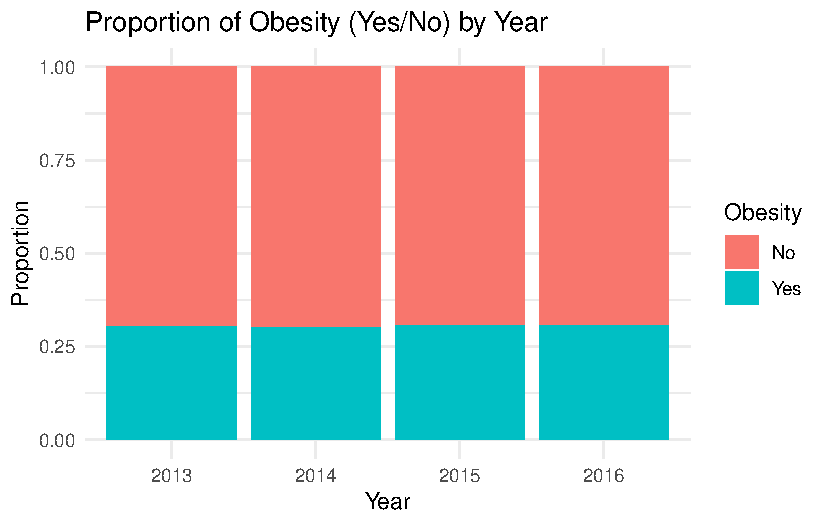
\includegraphics[keepaspectratio]{Group_Project_DA_files/figure-pdf/fig-obesityyear-1.pdf}}

}

\caption{\label{fig-obesityyear}Proportion of Obesity by Year}

\end{figure}%

Figure~\ref{fig-obesityyear} displays the proportion of Obesity by the
each year the questionnaire has been taken. There appears to be very
little if any difference in the change of obesity levels over the years.

\begin{figure}

\centering{

\pandocbounded{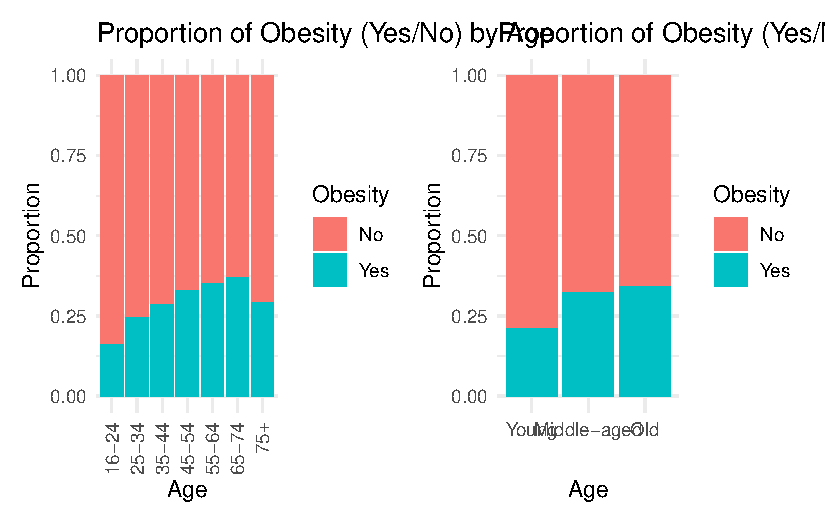
\includegraphics[keepaspectratio]{Group_Project_DA_files/figure-pdf/fig-ages-1.pdf}}

}

\caption{\label{fig-ages}Obesity Proportions against Age Groups and Age
Categories}

\end{figure}%

We look at Figure~\ref{fig-ages} to see if there is a significant
relationship between obesity and age, i.e.~can the age of a person
change their likelihood of being obese. The bar plot does indicate an
increase in obesity as age increases however it then drops in the last
category (75+). The difference in ages is made clearer in the right hand
plot where the age catgeories have been refined, and we see that young
people are least likely to be obese, middle aged are much more likely to
be obese and elderly are the most likely to be obese.

Figure~\ref{fig-gender} is a barplot being used to see if there is a
difference in obesity dependent on the gender of a person. The plot
shows there is actually a slight difference in gender and obesity
levels. There is a larger proportion of women who are obese suggesting
if gender is female they are slightly more likely to be obese than men.

\begin{figure}

\centering{

\pandocbounded{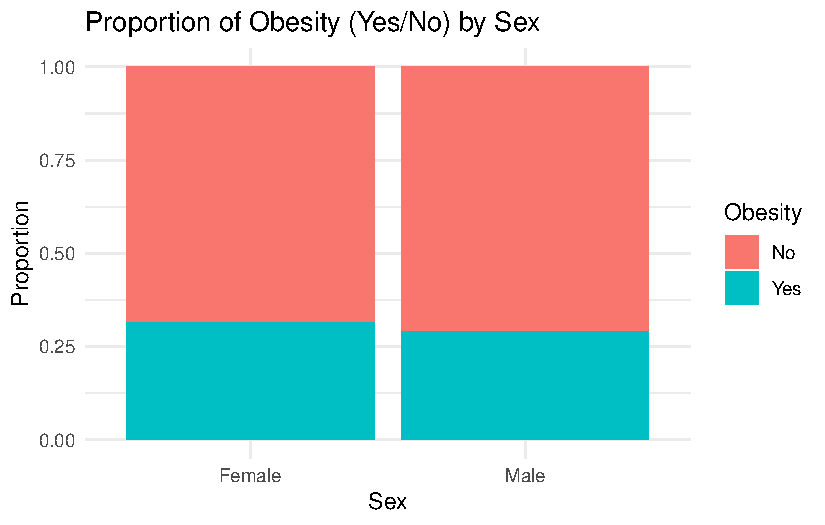
\includegraphics[keepaspectratio]{Group_Project_DA_files/figure-pdf/fig-gender-1.pdf}}

}

\caption{\label{fig-gender}Proportion of Obesity by Gender}

\end{figure}%

\begin{figure}

\centering{

\pandocbounded{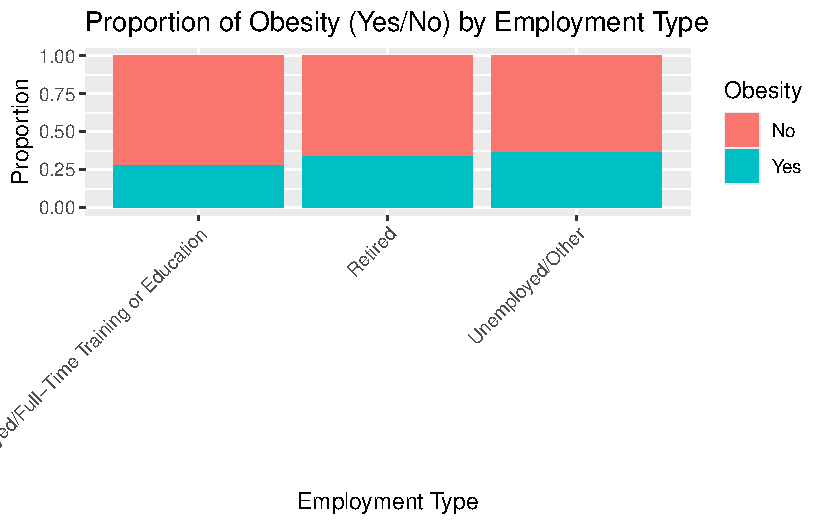
\includegraphics[keepaspectratio]{Group_Project_DA_files/figure-pdf/fig-social-1.pdf}}

}

\caption{\label{fig-social}Proportion of Obesity by Employment Type}

\end{figure}%

Figure~\ref{fig-social} refers to the Obesity rates of those
participating in the survey and their socio-economic status. This has
been refined into three categories, `employed/full time education',
`retired', `unemployed/other'. We can see that the least amount of
obesity occurs in the employed/full time education category, while the
category with highest obesity rates is the unemployed/other category
which is interesting when compared to the age graphs previously as we
might have expected retired to have the highest rates as the older age
catgories seemed to have higher obesity rates.

\begin{figure}

\centering{

\pandocbounded{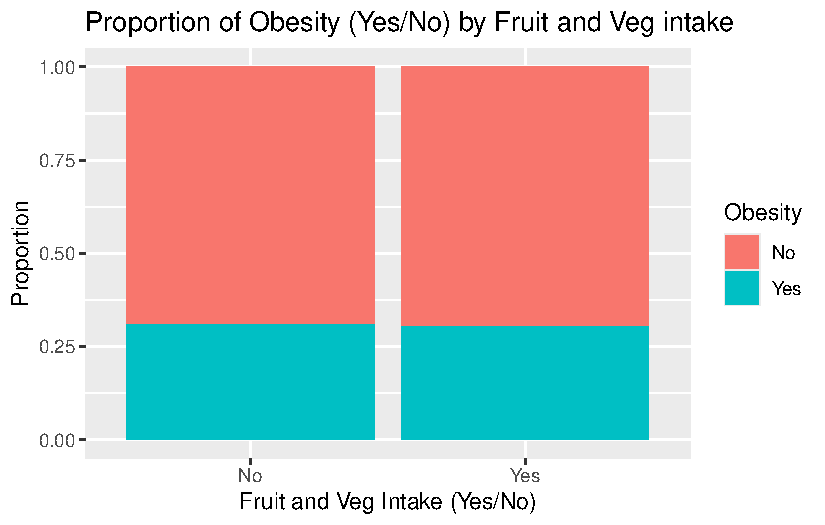
\includegraphics[keepaspectratio]{Group_Project_DA_files/figure-pdf/fig-FV-1.pdf}}

}

\caption{\label{fig-FV}The Proportion of Obesity Against Consumption of
the Required Amount of Fruit or Vegetables}

\end{figure}%

Figure~\ref{fig-FV} displays a barplot of Obesity rates vs if surveyed
people ate the correct amount of fruit and vegetables in a day
(lifestyle factors). We might have expected this to show there is a
significant impact on obesity rates if people ate their `5 a day'
however there seems to be no difference in obesity depending on a
persons fruit and veg intake.

\section{Formal Analysis}\label{sec-FA}

We start by fitting the full regression model containing all explanatory
variables. Since our response variable is binary, we fit a logistic
regression model. The full model can be written as: MENTION WHY NOT
DOING INTERACTION TERMS?

\[
Obese \sim Bernoulli(p_i)
\]

\[
logit(p_i)= \alpha + \beta_{\text{sex}}\cdot\mathbb{I}_{\text{sex}} + \beta_{\text{year}}\cdot\text{Year} + \beta_{\text{fv}}\cdot\mathbb{I}_{\text{FV}} + \beta_{\text{middle-aged}}\cdot\mathbb{I}_{\text{middle-aged}} + \beta_{\text{old}}\cdot\mathbb{I}_{\text{old}} + \beta_{retired}\cdot\mathbb{I}_{\text{retired}} + \beta_{unemployed}\cdot\mathbb{I}_{\text{unemployed}}
\]

where \(p_i\) is the probability of being obese and

\begin{itemize}
\item
  \(\alpha\) is the intercept (the baseline log-odds of obesity when all
  predictors are at their reference category),
\item
  \(\beta_\text{sex}\) is the coefficient for sex,
\item
  \(\mathbb{I}_{\text{sex}}(x)\) is an indicator function such that
\end{itemize}

\[
    \mathbb{I}_{\mbox{male}}(x) =
    \begin{cases}
    1 & \mbox{if gender of } x \mbox{ is male}, \\
    0 & \mbox{if gender of } x \mbox{ is female}.
    \end{cases}
\]

\begin{itemize}
\item
  \(\beta_\text{year}\) is the coefficient for survey year,
\item
  \(\beta_\text{fv}\) is the coefficient for whether an individual
  consumes the daily intake of either fruit, vegetables or both,
\item
  \(\mathbb{I}_{\text{FV}}(x)\) is an indicator function such that
\end{itemize}

\[
    \mathbb{I}_{\mbox{FV}}(x) =
    \begin{cases}
    1 & \mbox{if } x \mbox{ consumes the recommended daily intake of fruit and/or vegetables}, \\
    0 & \mbox{otherwise}.
    \end{cases}
\]

\begin{itemize}
\item
  \(\beta_\text{middle-aged}\) is the coefficient for being middle-aged
  (35-64 years old),
\item
  \(\mathbb{I}_{\text{middle-aged}}(x)\) is an indicator function such
  that
\end{itemize}

\[
    \mathbb{I}_{\mbox{middle-aged}}(x) =
    \begin{cases}
    1 & \mbox{if } x \mbox{ is middle-aged (35-64 years old)}, \\
    0 & \mbox{otherwise}.
    \end{cases}
\]

\begin{itemize}
\item
  \(\beta_\text{old}\) is the coefficient for being old (65+ years),
\item
  \(\mathbb{I}_{\text{old}}(x)\) is an indicator function such that
\end{itemize}

\[
    \mathbb{I}_{\mbox{old}}(x) =
    \begin{cases}
    1 & \mbox{if } x \mbox{ is old (65+ years old)}, \\
    0 & \mbox{otherwise}.
    \end{cases}
\]

\begin{itemize}
\item
  \(\beta_\text{retired}\) is the coefficient for being retired,
\item
  \(\mathbb{I}_{\text{retired}}(x)\) is an indicator function such that
\end{itemize}

\[
    \mathbb{I}_{\mbox{retired}}(x) =
    \begin{cases}
    1 & \mbox{if } x \mbox{ is retired}, \\
    0 & \mbox{otherwise}.
    \end{cases}
\]

\begin{itemize}
\item
  \(\beta_\text{unemployed}\) is the coefficient for being unemployed or
  in another non-working status,
\item
  \(\mathbb{I}_{\text{unemployed}}(x)\) is an indicator function such
  that
\end{itemize}

\[
    \mathbb{I}_{\mbox{unemployed}}(x) =
    \begin{cases}
    1 & \mbox{if } x \mbox{ is unemployed or in another non-working status}, \\
    0 & \mbox{otherwise}.
    \end{cases}
\]

PERHAPS SLIGHTLY REWORD AS I COPIED MAJORITY FROM THE EXAMPLE REPORT IN
WEEK 6? Stepwise regression with backward selection will be used to
determine whether the full model can be reduced based on the AIC. Hence,
the model which results in the lowest AIC will result in the final model
fitted to the data. In this case, the final model detailed below
provides the lowest AIC. The regression coefficients from the model are
displayed in Table~\ref{tbl-stepmod}.

\[
logit(p_i)= \alpha + \beta_{\text{sex}}\cdot\mathbb{I}_{\text{sex}} + \beta_{\text{middle-aged}}\cdot\mathbb{I}_{\text{middle-aged}} + \beta_{\text{old}}\cdot\mathbb{I}_{\text{old}} + \beta_{retired}\cdot\mathbb{I}_{\text{retired}} + \beta_{unemployed}\cdot\mathbb{I}_{\text{unemployed}}
\]

\begin{longtable}[]{@{}lll@{}}
\caption{Estimates of the fitted model's
coefficients.}\label{tbl-stepmod}\tabularnewline
\toprule\noalign{}
Term & Estimate (to 3 d.p.) & p-value (to 4 d.p.) \\
\midrule\noalign{}
\endfirsthead
\toprule\noalign{}
Term & Estimate (to 3 d.p.) & p-value (to 4 d.p.) \\
\midrule\noalign{}
\endhead
\bottomrule\noalign{}
\endlastfoot
Intercept & -1.340 & 0.0000 \\
Sex Male & -0.101 & 0.0069 \\
Middle-aged & 0.565 & 0.0000 \\
Old & 0.625 & 0.0000 \\
Retired & 0.104 & 0.1551 \\
Unemployed / Other & 0.401 & 0.0000 \\
\end{longtable}

INTERPRETING THE MODEL AND SEEING THIS VISUALLY IN Figure~\ref{fig-odds}

\begin{figure}

\centering{

\pandocbounded{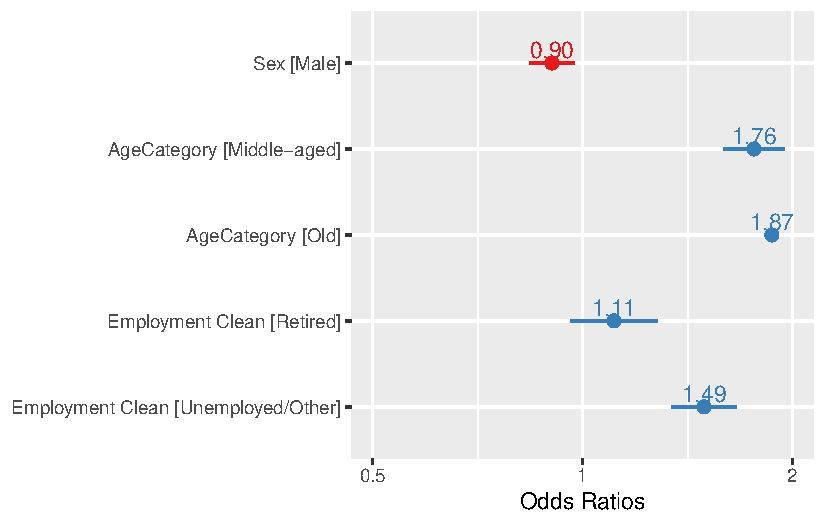
\includegraphics[keepaspectratio]{Group_Project_DA_files/figure-pdf/fig-odds-1.pdf}}

}

\caption{\label{fig-odds}Odds (Obesity)}

\end{figure}%

Figure~\ref{fig-odds} tells us
\ldots\ldots\ldots\ldots\ldots\ldots\ldots{} (FOCUS ON AGE AND
EMPLOYMENT AS MOST SIGNIFICANT?)

CHECKING THE MODEL WITH AIC AND Figure~\ref{fig-stepmoddiag} AND
Figure~\ref{fig-stepmodroc}.

\begin{figure}

\centering{

\pandocbounded{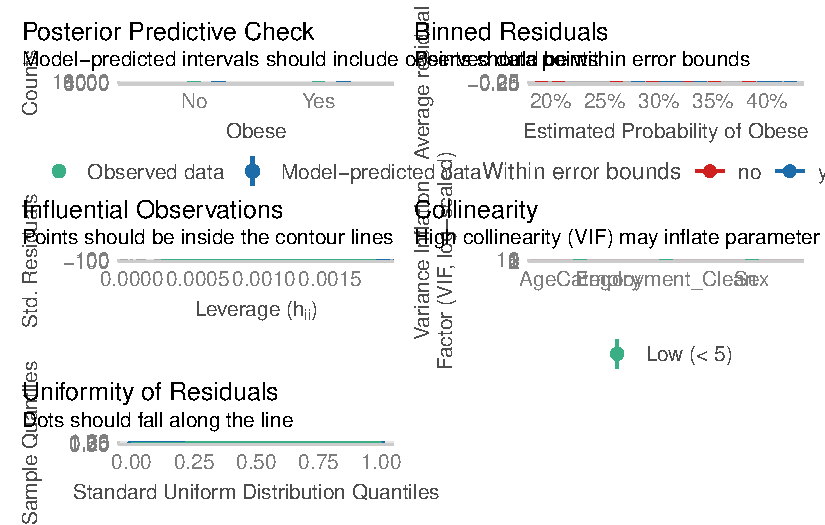
\includegraphics[keepaspectratio]{Group_Project_DA_files/figure-pdf/fig-stepmoddiag-1.pdf}}

}

\caption{\label{fig-stepmoddiag}GLM diagnostics for the obesity rates in
Scotland}

\end{figure}%

Figure~\ref{fig-stepmoddiag} allows us to assess if our model
assumptions are met. The posterior predictive check shows that the
model-predicted intervals include the observed data points. The binned
residuals plot highlight that the majority of points fall within the
error bounds however this does not appear to be 95\% of the
data\ldots\ldots\ldots\ldots..??????????? The influential observations
plot shows that all points are inside the contour lines. Finally, the
uniformity of residuals plot displays that the observed values do not
deviate from the model expectations when using simulated residuals. This
therefore demonstrates that our model is appropriately fitted to the
data.

MAYBE CUT AIC FOR FULL MODEL OR REWORD TO FOCUS ON THE REDUCED MODEL AND
INTERPRETING THIS: The reduced model has an AIC of 17009.35 compared to
the full model which has an AIC of 17011.99. This demonstrates that
although the reduced model has a lower AIC, the difference is
negligible.

\begin{figure}

\centering{

\pandocbounded{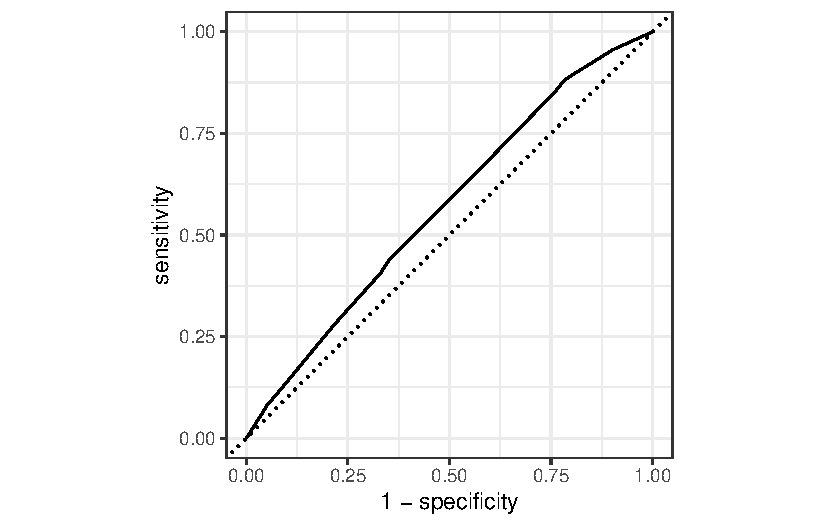
\includegraphics[keepaspectratio]{Group_Project_DA_files/figure-pdf/fig-stepmodroc-1.pdf}}

}

\caption{\label{fig-stepmodroc}ROC curve for Stepwise Regression Model}

\end{figure}%

To assess how good the model is at separating if a person is obese or
not, we will plot a ROC curve. This can be seen in
Figure~\ref{fig-stepmodroc}. Since the ROC curve is fairly close to the
diagonal line then this indicates that our model is only slighly better
than random guessing. Ideally we would want to see the ROC curve closer
to the top-left corner as this implies the model has high true positive
rates and low false positive rates.

Furthermore the ROC value is estimated at 0.432 which
demonstrates\ldots\ldots\ldots\ldots\ldots{} we need to improve model??

EXPAND ABOVE????

\section{Conclusions}\label{sec-con}

REWRITE (CUT A BIT) AND MAKE SURE APPROPRIATE FOR THE CHANGES WE MADE IN
THE FA SECTION.

This report has investigated trends in obesity prevalence in Scotland
over time and examined the impact of socio-economic factors using
logistic regression modeling. The findings indicate that obesity rates
have remained relatively stable, with no significant change over the
years, ALL ELSE CONSTANT? Furthermore, our model suggests that key
socio-economic factors, such as age and employment status, play a
crucial role in obesity prevalence. Specifically, being younger and
being employed, all else constant, is associated with lower odds of
obesity. In contrast, factors such as fruit and vegetable consumption
had minimal impact. This highlights the impact of socio-economic
conditions on health and the need \ldots\ldots..

The model diagnostics confirm that our regression model is appropriately
fitted to the data, with no major violations of model assumptions.
However, the ROC curve suggests that the model's predictive ability is
only slightly better than random guessing, indicating that additional
factors may be needed to better explain obesity prevalence.

CUT BELOW NOW ONLY DID STEPWISE? INSTEAD FOCUS ON THE ELIMINATION OF
YEAR AND FV: We also attempted to refine the model using stepwise
regression. While the reduced model achieved a marginally lower AIC, the
difference was negligible, and its predictive performance remained
similar to the full model. This suggests that while some variables could
be excluded without significant loss of explanatory power, the overall
findings remain consistent.

In conclusion, whilst obesity prevalence in Scotland has not changed
significantly over time, socio-economic factors, particularly age and
employment status, are important contributors. Future research could
explore additional lifestyle, behavioral, and environmental factors to
improve the predictive power of the model and gain deeper insights into
obesity trends and interventions.




\end{document}
